\chapter{MPTCP security}
\label{chap:mptcpsecurity}

\section{Threats analysis}
A complete security evaluation of MPTCP can be subdivided into two main categories:

\begin{itemize}
  \item A first perspective is to study the vulnerabilities in the current MPTCP design that can be exploited to carry out flooding or hijacking attacks on an MPTCP session. This is an assessment on how consistently the MPTCP extension would impact the security standards of a plain TCP connection;
  \item A second perspective is to understand how the new protocol affects the functioning and behavior of external security equipment. This evaluation might include compatibility issues for middleboxes not yet aware of MPTCP as well as more fundamental problematics related to monitoring solutions that wouldn't work anymore with MPTCP: by splitting the logic flow of data into different paths, potentially belonging to different ISPs, it would be much harder to keep track of the content of the transmitted data over the networks. Moreover, the MPTCP ability to reroute traffic on the fly, adding and removing addresses and interfaces, would per se cause major problems with current intrusion detection and intrusion prevention mechanisms.
\end{itemize}

This paper focuses on the first point: MPTCP enables data transmission using multiple source-destination address pairs per endpoint and this generates \textit{new} scenarios in which an attacker can exploit the way subflows are generated, maintained and destroyed to perform flooding or hijacking attacks. 
Flooding attacks are Denial-of-Service procedures that aim at overloading an MPTCP host with connection requests in order to quickly consume its resources.
Hijacking attacks aim at taking total control of the MPTCP session.

MPTCP security mechanism was designed with the primary goal of being at least as good as the one currently available for standard TCP \cite{rfc6181}. The official MPTCP documentation and analysis reports don't cover common threats affecting both TCP and MPTCP, but only the vulnerabilities introduced by the new protocol alone. Nevertheless, it is of paramount importance that the various security mechanisms deployed as part of standard TCP, for example mitigation techniques for reset attacks, are still compatible with Multipath TCP. Apart from the fundamental objective of keeping MPTCP at least as reliable and secure as TCP, official documents offer another set of requirements mainly related to securing subflow management in MPTCP. These requirements are \cite{rfc6824bis}:
\begin{itemize} 
\item Provide a mechanism to confirm that the parties in a subflow handshake are the same as in the original connection setup;
\item Provide verification that the peer can receive traffic at a new address before using it as part of a connection;
\item Provide replay protection, ensuring that a request to add/remove a subflow is fresh.
\end{itemize}

MPTCP involves an extensive usage of hash-based handshakes to achieve the required security specifications, as described in \autoref{chap:multipathtcp}. 

Once the security requirements are clear, it follows a set of related problematics due to the way MPTCP is added to the regular TCP stack. The entire behavior of the protocol relies on the TCP \textit{Options} field, which is of limited length of 40 bytes. This factor plays an important role in the definition of the security material to be exchanged during an MPTCP session (truncating the HMAC values and using shorter tokens are common techniques). Moreover, TCP \textit{Options} field has been designed to accept any custom protocol extending TCP and for security reasons many middleboxes would discard or modify packets containing unknown options. As a last point, MPTCP approach to subflow creation implies that a host cannot rely on other established subflows to support the addition of a new one \cite{rfc6182}: this last requirement follows the \textit{break-before-make} property of MPTCP, that must be able to react to a subflow failure a posteriori by establishing new subflows and automatically sending again the undelivered data. All these considerations define the fundamental boundaries and the context in which the security design of MPTCP has to be developed to meet the requirements.

\subsection{Threats classifications}
Introducing the support of multiple addresses per endpoint in a single TCP connection does result in additional vulnerabilities compared to single-path TCP. These new vulnerabilities need proper investigation in order to determine which of them can be considered critical and might require modifications in the protocol design in order to meet the required specifications. In order to classify how critical each security threat is, it is a good starting point to define the various typologies of attack according to their requirements, rate of success and what power they can provide to the attacker.
The general requirements for an attack to be executed might be grouped into the following categories \cite{rfc7430}:

\begin{itemize}  
\item \textit{Off-path attacker}: the attacker does not need to be located in any of the paths of the MPTCP connection at any time in order to execute the attack;
\item \textit{Partial-time (time-shifted) on-path attacker}: the attacker has to be able to eavesdrop a specific set of information during the lifetime of the MPTCP connection in order to execute the attack. It doesn't need to eavesdrop the entire communication in between the hosts, and the specific direction and subflow for the sniffing procedure are attack specific;
\item \textit{On-path attacker}: the attacker has to be on at least one of the paths during the entire lifetime of the MPTCP session in order to execute the attack.
\end{itemize}

The critical case is the one concerning off-path attacks, which do not require any eavesdrop procedure in order to be executed. In fact, on-path attacks are not considered part of the MPTCP work, since they allows for a significant number of attacks on regular TCP already. A primary goal in the design of MPTCP is not to introduce new ways to perform off-path attacks or time-shifted attacks.

The effects of an attack over an MPTCP connection and the power that the attack can provide to the attacker can be divided into two main categories \cite{rfc7430}:

\begin{itemize}  
\item \textit{Passive attacker}: the attacker is able to capture some or all of the packets of the MPTCP session but it can't manipulate, drop or delay them, and it can't inject new packets in the current session either;
\item \textit{Active attacker}: the attacker can pretend to be someone else, introduce new messages, delete existing messages, substitute one message for another, replay old messages, interrupt a communication's channel or alter stored information in a computer.
\end{itemize}

The rate of success of a certain attack over a MPTCP connection strongly depends on the specific requirements: two attacks falling in the same categories in terms of attacker eavesdrop capabilities and passive/active typologies might have rather different rates of success. For example, a certain kind of attack might require IP spoofing, thus being unfeasible in a network with ``ingress filtering'' \cite{rfc2827}.
There are no general thresholds to define when an attack can be considered a real threat according to the success rate, but this is an important factor to be studied in an attack analysis.

\section{Minor threats}
In this section are presented the minor residual threats for MPTCP under analysis by the IETF community at the time of writing, and all the related sections in this thesis closely follows such analysis as reported in the official document about security threats \cite{rfc7430}. Such vulnerabilities refer to the MPTCP version 0 specifications \cite{rfc6824}. By labeling certain vulnerabilities as ``minor'' it means they are considered acceptable in the process of moving MPTCP towards Standard Track. 

\subsection{DoS attack on MP\_JOIN}
This kind of DoS attack would prevent hosts from creating new subflows. In order to be executed, the attacker has to know a valid token value of an existing MPTCP session. This 32-bit value can be eavesdropped or the attacker has to guess it.
This attack exploits the fact that a host B receiving a SYN+MP\_JOIN message will create a state before answering with the SYN/ACK+MP\_JOIN packet. This means that some resources will be consumed at the host to keep in memory information regarding this connection request from the other party; in this way, when the host B receives the third ACK+MP\_JOIN packet, it can correctly associate it to the initial request and complete the handshake procedure. The creation of such state is required because there is no information in the ACK+MP\_JOIN packet that links it to the first SYN+MP\_JOIN request, so it is up to the host to save all the ongoing requests.
An attacker can exploit this by sending SYN+MP\_JOIN packets to a host without providing the final acknowledge packets. This can be done until the attacked host runs out of available spots for initiating additional subflows. The initial number of such available spots depends on the implementation and configuration at the host machine. 

This attack can be exploited to perform a typical TCP flooding attack. This is a good example of how MPTCP might introduce new vulnerabilities. 
SYN flooding attacks for TCP have been studied for many years and current implementations use mitigation techniques like SYN cookies \cite{rfc4987} in order to allow stateless connection initiations. But each SYN+MP\_JOIN packet received at the host would trigger the creation of an associated state, while this is not the case for the attacker machine that can simply forge these packet in stateless manner. Exploiting this unbalance in resource utilization is referred to as \textit{amplification attack}.

A possible solution to this problem is to extend the MP\_JOIN option format to include the information required to identify a specific request throughout the 3-way handshake, without requiring hosts to create associated states.

\subsection{Keys eavesdrop}
\label{keyseav}
An attacker can obtain the keys exchanged at the beginning of the MPTCP session, exploiting the fact that those are sent in clear. This is in fact a partial-time on-path eavesdropper attack, whose success would enable a vast set of attacking scenarios, even if the attacker itself has moved away from the session after sniffing the afore-mentioned keys.
The keys associated to an MPTCP session are sensitive pieces of information, used to identify a specific connection at the hosts and used as keying material for all the HMAC computations for the protocol. With such pieces of information an attacker can potentially execute a connection hijacking.  

The problem was acknowledged during the design of the first version of MPTCP, and considered acceptable. The maximum length of the TCP \textit{Options} field brings strong limitations for security implementations: for example, using certificates with the TCP options would be impossible. Moreover, strong cryptographic computation is also discouraged inside TCP for performance reasons. Nevertheless, some techniques can be used to prevent the keys' eavesdrop attack other than the more obvious possibility of adopting pre-shared keys. Such techniques are mentioned in the official documentation \cite{rfc7430}. Since this attack can affect security factors related to the main topic of this paper, namely ADD\_ADDR and ADD\_ADDR2, some of the proposed mitigation solutions are now presented in more details.

\subsubsection{Hash chains}
Hash chain is a way to obtain many one-time keys applying a cryptographic hash function recursively, starting from a random seed S:
  
  \[H[0] = H(S); H[1] = H(H[0]); H[2] = H(H[1]); ...; H[n] = H(H[n-1])\]
  
This technique allows to authenticate end hosts without the need to exchange keying material upfront. It is now reported the simplified scenario in which only host A needs to authenticate itself to host B. If host A initially identifies itself giving H[n], it can later on send H[n-1] for authentication towards host B. In fact, hash chains cannot be reversed (i.e. it is impossible to compute H[n-1] by just knowing H[n]), meaning only host A could have generated a valid H[n-1]; host B can verify its authenticity by simply hashing it and checking that it is equal to the previously seen H[n].
  The main issues with this operation is that, once H[n-1] is sent by host A, it cannot be reused, since this might have been eavesdropped, leading to a situation not dissimilar to the original problem. With key chains, hosts would continue traversing down the chain, meaning that a second authentication would require host A to send H[n-2] (of course, host A can calculate any value in the chain since it knows the original seed), and host B must have saved previously acknowledged H[n-1] to verify that H[H[n-1]] equals the received H[n-2] value.
  The main issue with this solution is that the value ``n'' will eventually reach 0, meaning that host A needs to compute a new hash chain from a new seed and also signal host B about this operation, thus requiring the definition of a new MPTCP option containing the final entry of the old chain (for authentication purposes) and the first entry of the new chain.
 Another direct consequence of such solution is that hash chains would add computational complexity to MPTCP operations, despite it being still reasonably acceptable.
 An unverified proposal for the new message exchange using hash chain can be found on the IETF mailing list \cite{hashchain}.
%\begin{figure}[!htb]
%\centering
%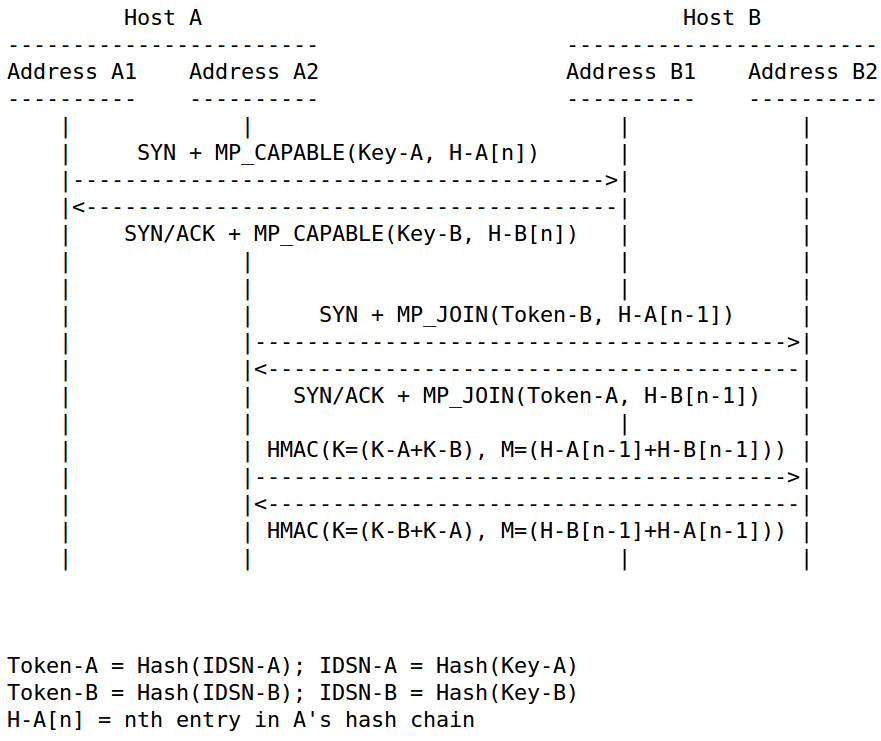
\includegraphics[width=0.75\textwidth]{images/hashchain}
%\caption{Hash chain message exchange proposal}
%\label{fig:hashchain}
%\end{figure}
In this proposal, four MP\_JOIN messages are exchanged in total for subflow addition: the first two messages are used for authentication purposes (the hash chain values are transmitted there together with the required tokens), but the last two messages operate in a similar fashion with respect to the current MPTCP solution, carrying an HMAC value whose key depends on the original keys exchanged via the MP\_CAPABLE option. In this way, eavesdropping the original keys is not enough to operate on the connection, but knowing the original keys is still required to validate subflows' creation.

\subsubsection{SSL/TLS and SSH}
Another well rated proposal to solve the keys' eavesdrop threat is to use application-layer protocols like SSL/TLS or SSH to negotiate a shared key between the endpoints. For example, SSL/TLS already provides a mechanism to negotiate shared secret by using a Diffie-Hellman algorithm, by exploiting asymmetric cryptographic computations \cite{rfc6101}, \textit{The Secure Sockets Layer (SSL) Protocol Version 3.0}. An RFC draft can be found to describe a possible prototype for this solution in MPTCP \cite{paasch-mptcp-ssl-00}. A bit field in the MP\_CAPABLE option would signal the intent of using keys provided by the application layer for the connection (maintaining backward compatibility with older versions of MPTCP that do not support this feature).
The main draw back of asking the application layer to provide the security mechanism, is that the application itself has to be upgraded to use the necessary MPTCP socket options:

\begin{itemize}
  \item MPTCP\_ENABLE\_APP\_KEY: when this option is enabled, MP\_CAPABLE is sent with the proper bit in order to signal the usage of an application supplied key for authentication;
  \item MPTCP\_KEY: this socket option is used to pass the actual key to the MPTCP layer.
\end{itemize}

Some synchronization concerns might arise due the fact that it's possible the client's application has already called the socket with the proper options while the server is still waiting for the key. In this case, temporarily dropping the SYN packets from the client, together with the usual TCP retransmission mechanism, should solve the problem.

\subsubsection{Secure MPTCP}
Secure MPTCT (SMTCP) refers to the integration of MPTCP with \textit{tcpcrypt} \cite{draft-bagnulo-mptcp-secure}, the latter being a protocol that attempts to encrypt almost the entire content of the traffic \cite{ietf-tcpinc-tcpcrypt-00}. SMTCP has been proposed as more secure version of MPTCP that would protect the data stream itself rather than addressing each and every security flaw in the signalling components of the protocol. Indeed, all the MPTCP signalling data would be encrypted and integrity protected as well, meaning that the overall protection for MPTCP would be achieved by the {tcpcrypt} extensions alone. An interesting factor of this solution, is that tcpcrypt also require sharing keying material to provide encryption, thus being tcpcrypt itself vulnerable to man-in-the-middle attacks during the initial key negotiation.

\subsection{SYN/ACK attack}
This is a partial-time on-path active attack. An attacker that can intercept and alter the MP\_JOIN packets is able to add any address it wants to the session. This is possible because there is no relation between the source addresses and the security material in the MP\_JOIN packets. But securing the source address in MP\_JOIN is not feasible if MPTCP is supposed to work through NATs, since they also operate in a similar manner over the source address in the packets, meaning that it is impossible to mitigate this attack without disrupting NATs' behavior by introducing modifications at the transport layer. Possible solutions have to reside on a different layer, perhaps securing the payload as a technique to limit the impact of such attack in a MPTCP session.

\section{ADD\_ADDR attack} 
\label{theaddaddrattack}
This paper is mainly focused on studying and testing the ADD\_ADDR vulnerability of MPTCP, as well as providing an analysis of the commonly accepted fix and its implementation in Linux Kernel. This section describes the attack procedure in details by following the corresponding analysis reported in the official documentation \cite{rfc7430}, while the considerations about the possible solutions for the ADD\_ADDR vulnerability as well as the implementation of the currently accepted solution can be found in \autoref{chap:addaddr2}. A simulated attack exploiting the vulnerability is reported in \autoref{chap:addaddrattackexecution}.

\subsection{Concept}
The ADD\_ADDR attack is an off-path active attack that exploits a major vulnerability in the MPTCP version 0. As previously mentioned, the attacks falling into this category are usually the most critical ones and can easily compromise the protocol security capabilities.
With the current MPTCP model, an attacker can forge and inject an ADD\_ADDR message into an MPTCP session to achieve a complete hijacking of the connection, placing itself as a man-in-the-middle. Being this an off-path attack, the attacker can conceptually send the forged ADD\_ADDR message from anywhere in the network (if allowed by routing), with no need to be physically close to the victim machines. At the end of the attacking procedure, the attacker will be able to operate in any way on the ongoing data transmission, with no clear warning given to the original parties involved in the MPTCP session.
% Add possible scenarios in which this could be dangerous
If no protection system is used at the application layer (like data encryption), the attacker can eavesdrop all the information and even modify or generate the exchanged content. The attack vector enabled by such exploit is huge and indeed not acceptable for the new protocol. For this reason, the ADD\_ADDR vulnerability is classified differently with respect to the minor threats listed in the previous section, and due to its characteristics it is considered a blocking issue in the MPTCP progress towards Standard Track \cite{rfc7430}.

\subsection{Procedure}
Let's consider a scenario in which two machines, host A and host B, are communicating over an MPTCP session involving one or more subflows. The attacker is called host C and it is operating remotely with no eavesdrop capabilities. The attacker is using address IPC and targeting a single MPTCP subflow between host A (address IPA and port PA) and host B (address IPB and port PB), even if other subflows might be operational. The scenario is reported in figure \ref{fig:attack1}.

\begin{figure}[!htb]
\centering
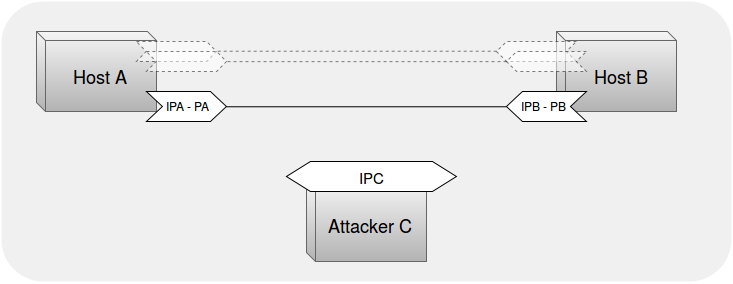
\includegraphics[width=0.8\textwidth]{images/Attack1}
\caption{ADD\_ADDR attack scenario}
\label{fig:attack1}
\end{figure}

Here is reported the procedure to carry out the ADD\_ADDR attack from a high-level perspective (the format of all the mentioned MPTCP option can be found in \autoref{chap:multipathtcp}):

%Consider adding images for each and every step of the attack

\begin{enumerate}  
\item  The first step performed by the attacker is to forge an ADD\_ADDR message as follows: it is an ACK TCP packet with source address IPA, destination address IPB and the advertised address in the ADD\_ADDR option is IPC. The ADD\_ADDR option also contains the address ID field, that cannot collide with existing identifiers for the ongoing subflows between hosts A and B. Even if the attacker cannot be certain about which value for address ID to use, high numbers are usually not already in use and shouldn't cause collision issues.
The forged packet is sent to host B.

\item Host B will process the forged packet as a legitimate request from host A of advertising a new available interface with address IPC. This most likely triggers the creation of a new subflow towards the new IP address, meaning that host B sends a SYN+MP\_JOIN packet to the attacker (in the case of the Linux implementation of MPTCP, the targeted host B has to be the client for the connection, since only the clients can open new subflows). This packet contains all the security material needed in the first phase of the MP\_JOIN three-way handshake, and the attacker does not need to operate over that portion of data: the attacker C simply manipulates the SYN+MP\_JOIN packet by changing the source IP to IPC and the destination IP to IPA; then, it forwards such packet to host A.

\item Host A will process the incoming packet as a legitimate request by host B of starting a new subflow from host B's new available interface having address IPC. All the required information is present in the MP\_JOIN option, like the token of host A that identifies the specific MPTCP session to which attach the new subflow to. Host A computes all the needed parameters (including a valid HMAC value), generates the SYN/ACK+MP\_JOIN packet and finally send it to IPC (which in reality belongs to the attacker). The attacker, similarly to the previous steps, manipulate the IP addresses of the packet from A by changing the source endpoint from IPA to IPC and the destination endpoint from IPC to IPB. At this point, attacker C sends the packet to host B.

\item All the parameters in the received packet looks correct to host B, which replies with an ACK+MP\_JOIN packet to attacker C. The attacker changes the source address to IPC and the destination address to IPA and sends the modified packet to host A. Upon acknowledge reception, host A will verify all the parameters in the packet (which will be correct since properly calculated by host B), and create a new subflow towards the address IPC. At this point the attacker has managed to place itself as man-in-the-middle.

\item As a further, optional step, the attacker can send RST packets to the other subflows in order to close them thus being able to perform a full hijack of the MPTCP session between host A and host B. The attacker can now operate upon the connection in any possible way, modifying, delaying, dropping, forging packets between the two parties.
\end{enumerate}

By exploit the ADD\_ADDR option, the attack procedure is relatively straightforward. Albeit there are some important requirements and limitations that consistently limit the rate of success of such attack, which are discussed in the next section (following the analysis in the official documentation \cite{rfc7430}).

\subsection{Requirements}
A first, basic prerequisite needed by the attacker to inject the ADD\_ADDR message into an ongoing MPTCP session is to know the IP addresses and port values adopted by host A and host B for the targeted subflow. It is reasonable to assume that the IP addresses are known. In a typical client-server configuration, the server's port for a certain application protocol is fixed and can be assumed to be known, too. For the client counterpart, the port value can cause problems in the presence of protection techniques like port randomization \cite{rfc6056}.

The knowledge about the above-mentioned 4-tuple is a basic requirement for obvious reasons, but knowing the endpoints' details is not enough to inject valid packets into an ongoing TCP session (that, in this case, can be also seen as an MPTCP subflow session): these packets have to contain sequence (SEQ) and acknowledgment (ACK) numbers that are compatible with the current ones within the stream. SEQ and ACK values are used in TCP to provide reliable, in-order transmission of data as well as services related to flow and congestion control. A very common protection technique is to randomize those 32-bit values at TCP connection setup, forcing the attacker (who acts off-path) to blindly guess them. TCP provides a window mechanism to deal with possible transmission's misalignments: at any given time, the accepted ACK values are those between the last ACK received and the same value plus the receiving window parameter. As a result, the number of packets to be sent in the attempt of guessing the right SEQ and ACK values and consequently the rate of success of the attack are strongly influenced by the TCP receive window size at the targeted TCP host.

The requirements listed so far all pertain to the underlying TCP protocol, whose validation mechanisms are still in place even for MPTCP subflows. The only MPTCP specific parameter that can cause the failure of the ADD\_ADDR attack procedure is the address ID field in the option. The purpose of this value has been previously explained, and it doesn't actually offer an overall protection improvement. It is enough for the attacker to chose an address ID value that is not in use by other subflow in the MPTCP session. In usual scenarios with a relatively limited number of subflows within the MPTCP session, applying a random value to this field (or a high number) should work just fine.

Moving away from the inner parameters evaluation and taking into consideration external protection mechanisms, it is worth mentioning that the attacker has to be able to manipulate and forge packets, including changing their source address field. This process, known as ``IP spoofing'', is a well known technique for which protection technologies have been developed, most notably the ``ingress filtering'' \cite{rfc2827} or the ``source address validation'' \cite{rfc7039}. However, these methods are not vastly deployed and cannot be considered a sufficient mitigation tool for the ADD\_ADDR vulnerability \cite{rfc7430}.

Lastly, the attacker has to be able to direct the malicious ADD\_ADDR packet to a host that is actually capable of starting a new subflow, namely the client in a client-server model. The current Linux Kernel implementation prohibits the server to instantiate a new subflow and only the client does so.
